\chapter{Overview\label{chap:2_body_tracking_overview}}

\section{Overview}

In Part~\ref{part:two} (with extensions in Parts~\ref{part:three} and \ref{part:four}) we will address the problem of inferring the 2D location of human joints in monocular RGB images - often called 2D body-pose detection. Recent approaches to this problem fall into two broad categories: 1) more traditional deformable part models \cite{modec} and 2) deep-learning based discriminative models \cite{deeppose, arjunaccv2014, jainiclr2014, tompson_efficient, tompsonnips2014}. Bottom-up part-based models are a common choice for this problem since the human body naturally segments into articulated parts. Traditionally these approaches have relied on the aggregation of hand-crafted low-level features such as SIFT~\cite{lowe1999object} or HoG~\cite{Dalal2005}, which are then input to a standard classifier or a higher level generative model. Care is taken to ensure that these engineered features are sensitive to the part that they are trying to detect and are invariant to numerous deformations in the input space (such as variations in lighting). On the other hand, discriminative deep-learning approaches learn an empirical set of low and high-level features which are typically more tolerant to variations in the training set and now outperform part-based models. However, incorporating priors about the structure of the human body (such as our prior knowledge about joint inter-connectivity) into such networks is difficult since the low-level mechanics of these networks is often hard to interpret. 

In this work we combine a ConvNet Part-Detector -- which alone outperformed all other existing methods at the time of publication~\cite{tompsonnips2014} -- with a part-based Spatial-Model into a unified learning framework. An overview of this architecture is shown in Figure~\ref{fig:overview_body_tracking}. In essence, this work is an attempt to combine the discriminative power of deep-learning with the inter-joint connectivity priors enforced by the more traditional deformable part models. In the first stage, we use a ConvNet to infer a probability distribution over spatial locations -- or heat-map -- describing the likelihood of each joint occurring in that spatial location (in Figure~\ref{fig:overview_body_tracking} there are 14 ground truth joints and so the ConvNet produces 14 heat-maps). The second stage graphical model inspired network then ``cleans up'' the noisy heat-map outputs to enforce correct inter-joint consistency.

\begin{figure}[th]
\centering
    \includegraphics[width=\columnwidth]{figures_2_body_tracking/overview}
    \caption{Network architecture overview}
  \label{fig:overview_body_tracking}
\end{figure}

Our translation-invariant ConvNet architecture utilizes a multi-resolution feature representation with overlapping receptive fields. Additionally, our Spatial-Model is able to approximate MRF loopy belief propagation, which is subsequently back-propagated through, and learned using the same learning framework as the Part-Detector. We show that the combination and joint training of these two models improves performance, and allows us to significantly outperform existing state-of-the-art models on the task of human body pose recognition.

\chapter{Architecture\label{chap:2_body_tracking_archiecture}}

\section{Model}

\subsection{Convolutional Network Part-Detector}
\label{sec:conv_model}
\begin{figure}[th]
\centering
    \includegraphics[width=\columnwidth]{figures_2_body_tracking/patch_model}
    \caption{Multi-Resolution Sliding-Window With Overlapping Receptive Fields}
  \label{fig:multiResPatchModel}
\end{figure}

The first stage of our detection pipeline is a deep ConvNet architecture for body part localization. The input is an RGB image containing one or more people and the output is a \emph{heat-map}, which produces a per-pixel likelihood for key joint locations on the human skeleton.

A \emph{sliding-window} ConvNet architecture is shown in Fig~\ref{fig:multiResPatchModel}. The network is slid over the input image to produce a dense heat-map output for each body-joint. Our model incorporates a \emph{multi-resolution} input with \emph{overlapping receptive fields}. The upper convolution bank in Fig~\ref{fig:multiResPatchModel} sees a standard 64x64 resolution input window, while the lower bank sees a larger 128x128 input context down-sampled to 64x64. The input images are then Local Contrast Normalized (LCN~\cite{torch7}) (after down-sampling with anti-aliasing in the lower resolution bank) to produce an approximate Laplacian pyramid. The advantage of using overlapping contexts is that it allows the network to see a larger portion of the input image with only a moderate increase in the number of weights. The role of the Laplacian Pyramid is to provide each bank with non-overlapping spectral content which minimizes network redundancy.

\begin{figure}[th]
  \centering
    \includegraphics[width=\columnwidth]{figures_2_body_tracking/oneshot_model}
    \caption{Efficient Sliding Window Model with Single Receptive Field}
  \label{fig:oneShotOneBank}
\end{figure}

An advantage of the Sliding-Window model (Fig~\ref{fig:multiResPatchModel}) is that the detector is translation invariant. However a major drawback is that evaluation is expensive due to redundant convolutions. Recent work~\cite{fastcnn,overfeatSermanet} has addressed this problem by performing the convolution stages on the full input image to efficiently create dense feature maps. These dense feature maps are then processed through convolution stages to replicate the fully-connected network at each pixel. An equivalent but efficient version of the sliding window model for a single resolution bank is shown in Fig~\ref{fig:oneShotOneBank}. Note that due to pooling in the convolution stages, the output heat-map will be a lower resolution than the input image.

For our Part-Detector, we combine an efficient sliding window-based architecture with multi-resolution and overlapping receptive fields; the subsequent model is shown in Fig~\ref{fig:oneShotMultiBank}. Since the large context (low resolution) convolution bank requires a stride of $\sfrac{1}{2}$ pixels in the lower resolution image to produce the same dense  output as the sliding window model, the bank must process four down-sampled images, each with a $\sfrac{1}{2}$ pixel offset, using shared weight convolutions. These four outputs, along with the high resolution convolution features, are processed through a 9x9 convolution stage (with 512 output features) using the same weights as the first fully connected stage (Fig~\ref{fig:multiResPatchModel}) and then the outputs of the low resolution bank are added and interleaved with the output of high resolution bank.

\begin{figure}[th]
  \centering
    \includegraphics[width=\columnwidth]{figures_2_body_tracking/one_shot_multires}
    \caption{Efficient Sliding Window Model with Overlapping Receptive Fields}
  \label{fig:oneShotMultiBank}
\end{figure}

While the above architecture gives optimal performance (and is exactly equivalent to the patch-based model), for our real-time system we simplify the above architecture by replacing the lower-resolution stage with a single convolution bank as shown in Fig~\ref{fig:oneShotMultiBankSimplified} and then upscale the resulting feature map. In all our practical implementation we use 3 resolution banks (but 2 banks are shown for brevity). Note that the simplified architecture is no longer equivalent to the original sliding-window network of Fig~\ref{fig:multiResPatchModel} since the lower resolution convolution features are effectively decimated and replicated leading into the fully-connected stage, however we have found empirically that the performance loss is minimal.

\begin{figure}[th]
  \centering
    \includegraphics[width=\columnwidth]{figures_2_body_tracking/one_shot_multires_ours}
    \caption{Approximation of Fig~\ref{fig:oneShotMultiBank}}
  \label{fig:oneShotMultiBankSimplified} 
\end{figure}

Supervised training of the network is performed using batched Stochastic Gradient Descent (SGD) with Nesterov Momentum. We use a Mean Squared Error (MSE) criterion to minimize the distance between the predicted output and a target heat-map. The target is a 2D Gaussian with a small variance and mean centered at the ground-truth joint locations. At training time we also perform random perturbations of the input images (randomly flipping and scaling the images) to increase generalization performance.

Note that an alternative model (such as in Tompson et al.~\cite{tompsonTOG14}) would replace the last 3 convolutional layers with a fully-connected neural network whose input context is the feature activations for the entire input image.  Such a model would be appropriate if we knew a priori that there existed a strong correlation between skeletal pose and the position of the person in the input frame since this alternative model is not invariant with respect to the translation of the person within the image.  However, the FLIC, LSP or MPII datasets have no such strong pose-location bias (i.e. a subject's torso is not always in the same location in the image), and therefore a sliding-window based architecture is more appropriate for our task.

\subsection{Higher-Level \emph{Spatial-Model}}
\label{sec:spatialmodel}

\begin{figure}[ht]
\centering
	\subcaptionbox{\footnotesize False Positive\label{fig:conv_net_fail_a}}{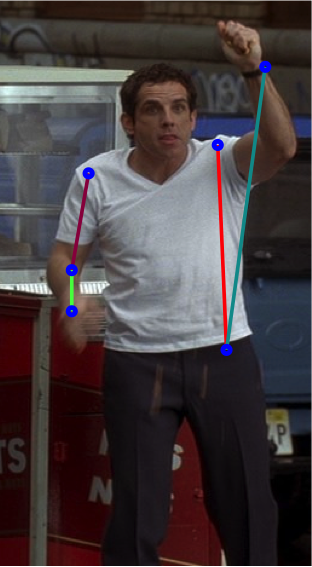
\includegraphics[height=5.5cm]{figures_2_body_tracking/part_detector_fail1}}
	\subcaptionbox{\footnotesize Multiple Subjects\label{fig:conv_net_fail_b}}{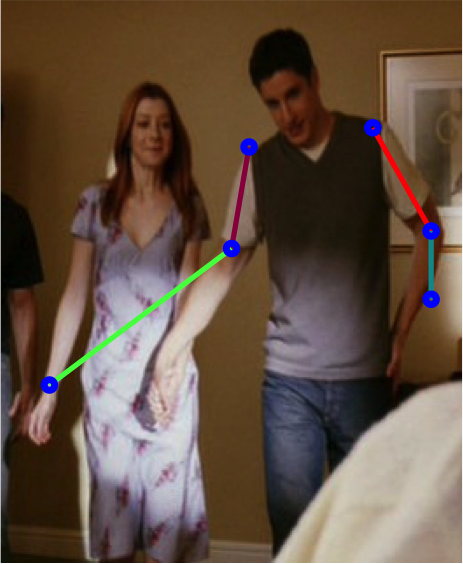
\includegraphics[height=5.5cm]{figures_2_body_tracking/part_detector_fail2}}
        \caption{ConvNet Part Detector Fail Cases}
        \label{fig:conv_net_fail}
\end{figure}

The Part-Detector (Section~\ref{sec:conv_model}) performance on our validation set predicts heat-maps that contain many false positives and poses that are anatomically incorrect; for instance when a peak for face detection is unusually far from a peak in the corresponding shoulder heat-map. Figures~\ref{fig:conv_net_fail_a} and \ref{fig:conv_net_fail_b} show two additional fail cases; 1) when a strong false positive outlier results in an incorrectly predicted joint location and 2) when strong activations from another subject in the frame result in an incorrectly labeled joint. Even in the presence of foreshortening, in both these cases it is clear that given the length of the correctly labeled limbs, one should be able to improve the prediction given that the incorrectly labeled limbs are anatomically incorrect.

In spite of the improved Part-Detector context (using our technique of overlapping receptive fields), the feed forward network still has difficulty learning an implicit model of the constraints of the body parts for the full range of body poses. We use a higher-level \emph{Spatial-Model} to constrain joint inter-connectivity and enforce global pose consistency. The expectation of this stage is to not increase the performance of detections that are already close to the ground-truth pose, but to remove false positive outliers that are anatomically incorrect.

\begin{figure}[th]
  \centering
    \includegraphics[width=0.6\columnwidth]{figures_2_body_tracking/mrf1}
    \caption{Linear chain MRF}
  \label{fig:mrf1} 
\end{figure}

Similar to Jain et al.~\cite{jainiclr2014}, we formulate the \emph{Spatial-Model} as an MRF model over the distribution of spatial locations for each body part.  The spatial model of \cite{jainiclr2014} is shown in Figure~\ref{fig:mrf1}. $\tilde{f}$, $\tilde{s}$, $\tilde{e}$, $\tilde{w}$, $f$, $s$, $e$, and $w$ are 2D random variables (or random Matrices), describing the likelihood of the face, shoulder, elbow and wrist joints for each pixel location in the input image \footnote{note that due to downsampling in the part detector this will be at a lower resolution than the input, and we use nearest-neighbor up-sampling to bring the heat-maps into the original resolution}. $\tilde{f}$, $\tilde{s}$, $\tilde{e}$ and $\tilde{w}$ are the noisy heat-maps from the ConvNet output (Section~\ref{sec:conv_model}) (or visible variables) and $f$, $s$, $e$, and $w$ are the clean heat-maps (or hidden variables) that we are trying to infer. Note that in practice, the full tree for the LSP dataset will include 14 nodes and the tree for the FLIC dataset will include 7 nodes, one node for each of the joints we are trying to infer.  For brevity only 4 nodes are shown.

$\phi(f)$, $\phi(s)$, $\phi(e)$ and $\phi(w)$ are the unary potentials (or sometimes called an image evidence function when the factor between the hidden and visible variables is a 2D tensor), and $\psi(f,s)$, $\psi(s,e)$ and $\psi(e,w)$ are the pair-wise factors describing the joint priors between adjacent neighbors in the linear chain-MRF. As we will see, these priors enforce inter-joint consistency.  Using these factors, we can describe the joint probability distribution as a product of factors, normalized by the partition function $Z$:

\begin{equation}
\bar{p}\left(f,s,e,w,\tilde{f},\tilde{s},\tilde{e},\tilde{w}\right) = \frac{1}{Z}\prod_{i,j}\psi\left(x_i,x_j\right)\prod_{k}\phi\left(x_k\right)
\label{eq:mrf1}
\end{equation}

The goal of our network is then to infer the distributions of the hidden variables $f$, $s$, $e$ and $w$ by marginalization of other variables in the joint distribution. One such method is to use a belief propagation formulation, which can be shown to converge to an exact solution given that the MRF in Figure~\ref{fig:mrf1} is a tree-structured graph. After a single round of belief propagation, the belief of a variable $x_i$ is given by the product of incoming messages from each neighbor joint $j$, $m_{ji}\left(x_i\right)$, multiplied by the unary factor for the joint $\psi\left(x_i\right)$: 

\begin{equation}
b\left(x_i\right)=k\phi\left(x_i\right)\prod_{j\in N(i)}m_{ji}\left(x_i\right) \\
\label{eq:mrf1_message_passing}
\end{equation}

Here $k$ is a normalizing partition function. Each incoming message from joint $j$ to joint $i$ is described by the product of incoming messages to joint $j$ from it's neighbors not including $i$ (i.e. in the set $N(j)-\{i\}$, where $N(j)$ is the set of adjacent neighbors for node $j$), multiplied with the marginalized product of the unary potential for node $j$, $\psi\left(x_j\right)$, and the pair-wise factor between $i$ and $j$, $\psi\left(x_j, x_i\right)$:

\begin{equation}
m_{ji}\left(x_i\right) \leftarrow \sum_{x_j}\phi\left(x_j\right)\psi\left(x_j,x_i\right)\prod_{k\in N(j) - \{i\}}m_{kj}\left(x_j\right)
\end{equation}

Since the height of our tree is 3, it can also be shown that message passing will converge to the exact solution after 3 rounds. Writing out the full expression for the marginalization of the hidden variable for the face joint we get:

\begin{equation}
b\left(f\right)=k\phi(f)\sum_s \phi(s)\psi(s,f)\sum_e \phi(e)\psi(e,s) \sum_w \phi(w)\psi(w,e)
\label{eq:face_marginal}
\end{equation}

Note that we can also arrive at the same solution by marginalizing the joint distribution of Equation~\ref{eq:mrf1}, however the belief propagation formulation provides us with invaluable insight as to the function of the pair-wise prior as we will show. Note that the expression in Equation~\ref{eq:face_marginal}, requires sequential calculation of a 4D tensor and 2D tensor products (for the multiplication of the pairwise and unary potentials), which is then integrated over 2D to calculate the marginalized message distribution. To re-phrase the above formation so that it is more amenable to implementation as a neural network, we simplify Equation~\ref{eq:face_marginal}:

\begin{equation}
b\left(f\right)\approx k\phi(f)\prod_i\sum_{x_i} \phi(x_i)\psi(x_i,f)
\label{eq:face_marginal_simple}
\end{equation}

This means that rather than sequentially taking each product and multiplying before marginalizing, the messages from adjacent joints can be calculated in parallel, which as we shall see, is easier to implement as a single layer of neural network. However, by doing so we have actually changed the structure of the MRF; the new formulation is a star graph as shown in Figure~\ref{fig:mrf2} (visible nodes are not shown for brevity).

\begin{figure}[th]
  \centering
    \includegraphics[width=\columnwidth]{figures_2_body_tracking/mrf2}
    \caption{Star MRF}
  \label{fig:mrf2} 
\end{figure}

Note that Equation~\ref{eq:face_marginal_simple} is effectively a separate star graph for each of the joint marginals that we will calculate, i.e. the marginalized hidden variable we infer for the face joint, is not the same as the variable we use for the shoulder joint.  Also not that we have weakened our pair-wise priors; instead of modeling the tight coupling between the shoulder and wrist, when incorporating evidence for marginalization of the face, instead we will model the much looser pair-wise distribution of the wrist to face joint. Since the average displacement between the face and wrist joint is large, the prior distribution will not have high entropy and will therefore have a smaller impact on the marginalized face distribution.

The 4D $\times$ 2D tensor product of the pairwise and unary factors as written in Equation~\ref{eq:face_marginal_simple} is extremely expensive to calculate. We therefore make one important approximation, instead of performing the tensor product then marginalizing, we instead replace this with a convolution operator and use a `conditional pairwise' factor as shown in Equation~\ref{eq:conv_prior}. By doing so our implicit assumption is that the distribution of a joint`s location given the location of another joint is independent of the position in the input image, i.e., the expected displacement between joints is the same and is independent of the limb`s position in the image. In our model this is a fair assumption for 2 reasons: 1) we expect that the movement of a joint is independent of the person`s location in an image and 2) we want to formulate a detector architecture that is translation invariant and so modeling the full factor as a convolutional prior will achieve this.

\begin{equation}
b^\prime\left(f\right)\approx k\phi(f)\prod_i \phi(x_i)\ast\psi(x_i|f)
\label{eq:conv_prior}
\end{equation}

Note that this new formulation is no longer a traditional MRF, however it is still a graphical model that is able to capture the inter-dependancies between joints.  Lastly, we add a scalar bias term, $b_{x_i|j}$, to each of the messages:

\begin{equation}
b^\prime\left(f\right)\approx k\phi(f)\prod_i \phi(x_i)\ast\psi(x_i|f) + b_{x_i|f}
\label{eq:final_equation}
\end{equation}

This bias essentially sets a background probability distribution. This bias is extremely important since the ConvNet may output false negatives, particularly for difficult joints like the wrist and ankle, which results in a product with a zero probability, causing strong positive activations for neighbor joints to be incorrectly attenuated. The ratio between the dynamic range of the conditional prior and the strength of the bias term sets how much a neighbor joint ``trusts" the incoming message, and for strongly coupled joints (like the face and shoulder), we indeed find that the network learns to set the background bias close to zero during training. In contrast, for loosely coupled joints (such as wrist and face), the network will learn to set the bias high and the dynamic range of the prior term small.

Fig~\ref{fig:heat_map_examples} shows a practical example of how the Spatial-Model is able to remove an anatomically incorrect strong outlier from the face heat-map by incorporating the presence of a strong shoulder detection. For simplicity, only the shoulder and face joints are shown, however, this example can be extended to incorporate all body part pairs. If the shoulder heat-map shown in Fig~\ref{fig:heat_map_examples} had an incorrect false-negative (i.e. no detection at the correct shoulder location), the addition of the background bias $b_{v\rightarrow A}$ would prevent the output heat-map from having no maxima in the detected face region.

\begin{figure}[th]
  \centering
    \includegraphics[width=\columnwidth]{figures_2_body_tracking/spatial}
    \caption{Didactic Example of Message Passing Between the Face and Shoulder Joints}
  \label{fig:heat_map_examples}
\end{figure}

Fig~\ref{fig:heat_map_examples} contains the conditional distributions for face and shoulder parts learned on the FLIC~\cite{modec} dataset. For any part $x_i$ the distribution $\psi\left(x_i,x_j\right)$ is the identity map, and so the message passed from any joint to itself is its unary distribution. Since the FLIC dataset is biased towards front-facing poses where the right shoulder is directly to the lower right of the face, the model learns the correct spatial distribution between these body parts and has high probability in the spatial locations describing the likely displacement between the shoulder and face. For datasets that cover a larger range of the possible poses (for instance the LSP~\cite{Johnson10} dataset), we would expect these distributions to be less tightly constrained, and therefore this simple Spatial-Model will be less effective. 

For our practical implementation we treat the distributions above as energies to avoid the evaluation of $k$ in Equation~\ref{eq:final_equation}. There are 3 reasons why we do not include the partition function. Firstly, we are only concerned with the maximum output value of our network, and so we only need the output energy to be proportional to the normalized distribution. Secondly, since both the part detector and spatial model parameters contain only shared weight (convolutional) parameters that are equal across pixel positions, evaluation of the partition function during back-propagation will only add a scalar constant to the gradient weight, which would be equivalent to applying a per-batch learning-rate modifier. Lastly, since the number of parts is not known a priori (since there can be unlabeled people in the image), and since the distributions $p_v$ describe the part location of a single person, we cannot normalize the Part-Model output. Our final model is a modification to Eq~\ref{eq:final_equation}:

\begin{align}
\label{eq:mrf2}
\bar{e}_A = \operatorname{exp}\left(\sum_{v\in V}\left[\operatorname{log}\left(\operatorname{SoftPlus}\left(e_{A|v}\right) \ast \operatorname{ReLU}\left(e_v\right) + \operatorname{SoftPlus}\left(b_{v\rightarrow A}\right)\right)\right]\right) \\
\text{where: } \operatorname{SoftPlus}\left(x\right) = \sfrac{1}{\beta} \operatorname{log}\left(1+\operatorname{exp}\left(\beta x\right)\right)\text{, } \sfrac{1}{2} \leq\beta\leq 2 \notag \\
\operatorname{ReLU}\left(x\right) = \operatorname{max}\left(x, \epsilon \right)\text{, } 0<\epsilon\leq 0.01\notag
\end{align}

The network-based implementation of Eq~\ref{eq:mrf2} is shown in Fig~\ref{fig:spatial_model_network}. Eq~\ref{eq:mrf2} replaces the outer multiplication of Eq~\ref{eq:final_equation} with a log space addition to improve numerical stability and to prevent coupling of the convolution output gradients (the addition in log space means that the partial derivative of the loss function with respect to the convolution output is not dependent on the output of any other stages). However, this then requires that our output criterion be before the outer exp, however for visualization the exp is required. The inclusion of the \emph{SoftPlus} and \emph{ReLU} stages on the weights, biases and input heat-map maintains a strictly greater than zero convolution output, which prevents numerical issues for the values leading into the \emph{Log} stage. Finally, a \emph{SoftPlus} stage is used to maintain continuous and non-zero weight and bias gradients during training. With this modified formulation, Eq~\ref{eq:mrf2} is trained using back-propagation and SGD.

\begin{figure}[th]
  \centering
    \includegraphics[width=\columnwidth]{figures_2_body_tracking/spatial_model}
    \caption{Single Round Message Passing Network}
  \label{fig:spatial_model_network}
\end{figure}

The convolution sizes are adjusted so that the largest joint displacement is covered within the convolution window. For our 90x60 pixel heat-map output, this results in large 128x128 convolution kernels to account for a joint displacement radius of 64 pixels (note that padding is added on the heat-map input to prevent pixel loss). Therefore for such large kernels we use FFT convolutions based on the GPU implementation by Mathieu et al.~\cite{fft}.

The convolution weights are initialized using the empirical histogram of joint displacements created from the training examples. This initialization improves learned performance, decreases training time and improves optimization stability. During training we randomly flip and scale the heat-map inputs to improve generalization performance.

The FLIC and LSP datasets contain many frames with more than a single person, while the joint locations from only one person in the scene are labeled. Therefore an approximate torso bounding box is provided at test time for the single labeled person in the scene. We incorporate this data by including an extra ``torso-joint heat-map" to the input of the Spatial-Model so that it can learn to select the correct feature activations in a cluttered scene as shown in Figure~\ref{fig:torso_input}.

\begin{figure}[th]
  \centering
    \includegraphics[width=0.8\columnwidth]{figures_2_body_tracking/torso_input}
    \caption{Torso heat-map utilization}
  \label{fig:torso_input}
\end{figure}

\subsection{Unified Model}
\label{sec:unified}

Since our Spatial-Model (Section~\ref{sec:spatialmodel}) is trained using back-propagation, we can combine our Part-Detector and Spatial-Model stages in a single \emph{Unified Model}. To do so, we first train the Part-Detector separately and store the heat-map outputs. We then use these heat-maps to train a Spatial-Model. Finally, we combine the trained Part-Detector and Spatial-Models and back-propagate through the entire network.

This unified fine-tuning further improves performance. We hypothesize that because the Spatial-Model is able to effectively reduce the output dimension of possible heat-map activations, the Part-Detector can use available learning capacity to better localize the precise target activation.

\chapter{Experimental Results\label{chap:2_body_tracking_experimental}}

\section{Results}

The models from Sections \ref{sec:conv_model} and \ref{sec:spatialmodel} were implemented within the Torch7~\cite{torch7} framework (with custom GPU implementations for the non-standard stages above). Training the Part-Detector takes approximately 48 hours, the Spatial-Model 12 hours, and forward-propagation for a single image through both networks takes 51ms \footnote{We use a 12 CPU workstation with an NVIDIA Titan GPU}.

\begin{figure}[th]
  \centering
    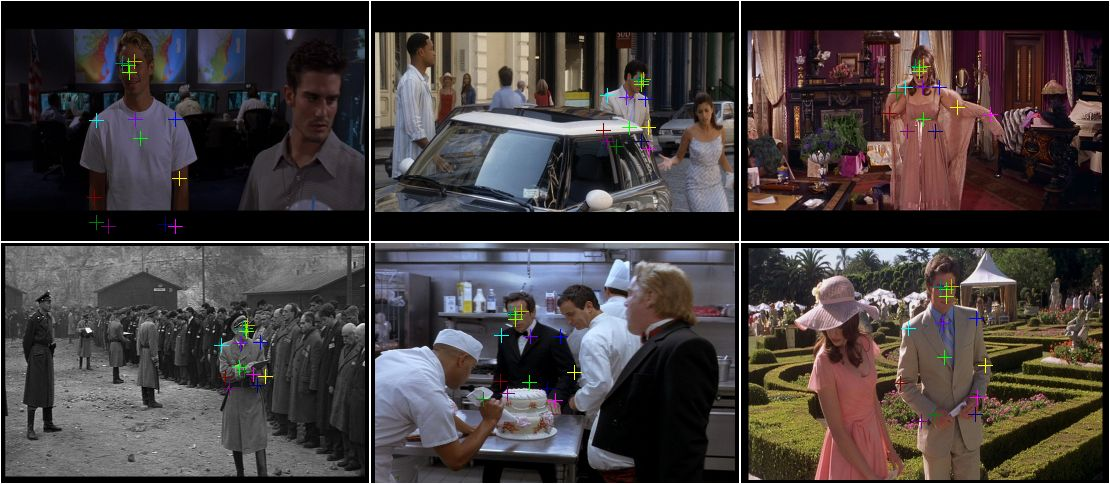
\includegraphics[width=\columnwidth]{figures_2_body_tracking/flic_plus_sample}
    \caption{Sample images from FLIC-plus dataset}
  \label{fig:flic_plus}
\end{figure}

We evaluated our architecture on the FLIC~\cite{modec} and extended-LSP~\cite{Johnson10} datasets. These datasets consist of still RGB images with 2D ground-truth joint information generated using Amazon Mechanical Turk. The FLIC dataset is comprised of 5003 images from Hollywood movies with actors in predominantly front-facing standing up poses (with 1016 images used for testing), while the extended-LSP dataset contains a wider variety of poses of athletes playing sport (10442 training and 1000 test images).

The FLIC-full dataset contains 20928 training images, however many of these training set images contain samples from the 1016 test set scenes and so would allow unfair over-training on the FLIC test set. Therefore, we propose a new dataset - called \emph{FLIC-plus} (\href{http://cims.nyu.edu/~tompson/flic_plus.htm}{http://cims.nyu.edu/$\sim$tompson/flic\_plus.htm}) - which is a 17380 image subset from the FLIC-plus dataset. Sample images from this dataset are shown in Figure~\ref{fig:flic_plus}. To create this dataset, we produced unique scene labels for both the FLIC test set and FLIC-plus training sets using Amazon Mechanical Turk. We then removed all images from the FLIC-plus training set that shared a scene with the test set. Since 253 of the sample images from the original 3987 FLIC training set came from the same scene as a test set sample (and were therefore removed by the above procedure), we added these images back so that the FLIC-plus training set is a superset of the original FLIC training set. Using this procedure we can guarantee that the additional samples in FLIC-plus are sufficiently independent to the FLIC test set samples.

For evaluation of the test-set performance we use the measure suggested by Sapp et. al.~\cite{modec}. For a given normalized pixel radius (normalized by the torso height of each sample) we count the number of images in the test-set for which the distance of the predicted UV joint location to the ground-truth location falls within the given radius.

Fig~\ref{fig:flic_elbow} and \ref{fig:flic_wrist} show our model's performance on the the FLIC test-set for the elbow and wrist joints respectively and trained using both the FLIC and FLIC-plus training sets. Performance on the LSP dataset is shown in Fig~\ref{fig:lsp_best} and \ref{fig:lsp_best_lower}. For LSP evaluation we use person-centric (or non-observer-centric) coordinates for fair comparison with prior work~\cite{deeppose,dantone13cvpr}. Our model outperforms existing state-of-the-art techniques on both of these challenging datasets with a considerable margin.

\begin{figure}[th]
  \centering
  \begin{subfigure}[b]{0.63\textwidth}
    \begin{subfigure}[b]{0.99\textwidth}
         % Trim is left, bottom, right, top
          \begin{flushright}
                  \includegraphics[trim=0cm 0.6cm 1.1cm 0.6cm, clip=true, width=0.95\textwidth]{figures_2_body_tracking/flic_legend.pdf}
          \end{flushright}
      \end{subfigure}
    \hfill

    \begin{subfigure}[b]{0.49\textwidth}
          \includegraphics[width=\textwidth]{figures_2_body_tracking/best_flic_elbow.pdf}
          \caption{FLIC: Elbow}
          \label{fig:flic_elbow}
    \end{subfigure}
    \begin{subfigure}[b]{0.49\textwidth}
          \includegraphics[width=\textwidth]{figures_2_body_tracking/best_flic_wrist.pdf}
          \caption{FLIC: Wrist}
          \label{fig:flic_wrist}
    \end{subfigure}
  \end{subfigure}
  \begin{subfigure}[b]{0.307\textwidth}
        \includegraphics[width=\textwidth]{figures_2_body_tracking/best_lsp.pdf}
        \caption{LSP: Wrist and Elbow}
        \label{fig:lsp_best}
  \end{subfigure}
  \caption{Model Performance}
  \label{fig:flic_results}
\end{figure} 

Fig~\ref{fig:spatial_model_performance} illustrates the performance improvement from our simple Spatial-Model. As expected the Spatial-Model has little impact on accuracy for low radii threshold, however, for large radii it increases performance by 8 to 12\%. Unified training of both models (after independent pre-training) adds an additional 4-5\% detection rate for large radii thresholds. 

\begin{figure}[th]
  \centering
  \begin{subfigure}[b]{0.31\textwidth}
        \includegraphics[width=\textwidth]{figures_2_body_tracking/best_lsp_lower.pdf}
        \caption{LSP: Ankle and Knee}
        \label{fig:lsp_best_lower}
  \end{subfigure}
  \begin{subfigure}[b]{0.31\textwidth}
        \includegraphics[width=\textwidth]{figures_2_body_tracking/spatial_model_performance.pdf}
        \caption{FLIC: Wrist}
        \label{fig:spatial_model_performance}
  \end{subfigure}
  \begin{subfigure}[b]{0.31\textwidth}
        \includegraphics[width=\textwidth]{figures_2_body_tracking/banks.pdf}
        \caption{FLIC: Wrist}
        \label{fig:banks}
  \end{subfigure} 
  \caption{(a) Model Performance (b) With and Without Spatial-Model (c) Part-Detector Performance Vs Number of Resolution Banks (FLIC subset)}
  \label{fig:lsp_results_1}
\end{figure}

The impact of the number of resolution banks is shown in Fig~\ref{fig:banks}). As expected, we see a big improvement when multiple resolution banks are added. Also note that the size of the receptive fields as well as the number and size of the pooling stages in the network also have a large impact on the performance. We tune the network hyper-parameters using coarse meta-optimization to obtain maximal validation set performance within our computational budget (less than 100ms per forward-propagation).

Fig~\ref{fig:pics} shows the predicted joint locations for a variety of inputs in the FLIC and LSP test-sets. Our network produces convincing results on the FLIC dataset (with low joint position error), however, because our simple Spatial-Model is less effective for a number of the highly articulated poses in the LSP dataset, our detector results in incorrect joint predictions for some images. We believe that increasing the size of the training set will improve performance for these difficult cases.
% Source images are 720x480 or 1.5:1 aspect ratio --> We want the output aspect ratio to be 0.7058:1

\begin{figure}[th]
  \centering
  \adjustbox{trim={0.2\width} {0.075\height} {0.475\width} {.2\height},clip,height=0.256\textwidth}% Trim is left bottom right top
      {\includegraphics[width=\textwidth]{figures_2_body_tracking/pred_along-came-polly-00117171_02592.pdf}}
  \adjustbox{trim={0.0\width} {0.15\height} {0.6\width} {.1\height},clip,height=0.256\textwidth}
      {\includegraphics[width=\textwidth]{figures_2_body_tracking/pred_bend-of-the-river-00116721_06712.pdf}}
  \adjustbox{trim={0.2\width} {0.15\height} {0.5\width} {.2\height},clip,height=0.256\textwidth}
      {\includegraphics[width=\textwidth]{figures_2_body_tracking/pred_funny-girl-dvd-video-00184781_09440.pdf}}
  \adjustbox{trim={0.01\width} {0.15\height} {0.575\width} {.15\height},clip,height=0.256\textwidth}
      {\includegraphics[width=\textwidth]{figures_2_body_tracking/pred_funny-girl-dvd-video-00187111_09513.pdf}}
  \adjustbox{trim={0.275\width} {0.125\height} {0.375\width} {.15\height},clip,height=0.256\textwidth}
      {\includegraphics[width=\textwidth]{figures_2_body_tracking/pred_hitch-00155861_12551.pdf}}

  \centering
  \adjustbox{trim={0.35\width} {0.0\height} {0.35\width} {0.05\height},clip,height=0.315\textwidth}
      {\includegraphics[width=\textwidth]{figures_2_body_tracking/pred_im1036.pdf}}
  \adjustbox{trim={0.4\width} {0.0\height} {0.42\width} {0.05\height},clip,height=0.315\textwidth}
      {\includegraphics[width=\textwidth]{figures_2_body_tracking/pred_im1112.pdf}}
  \adjustbox{trim={0.32\width} {0.0\height} {0.34\width} {0.1\height},clip,height=0.315\textwidth}
      {\includegraphics[width=\textwidth]{figures_2_body_tracking/pred_im1072.pdf}}
  \adjustbox{trim={0.3\width} {0.05\height} {0.34\width} {.1\height},clip,height=0.315\textwidth}
      {\includegraphics[width=\textwidth]{figures_2_body_tracking/pred_im1143.pdf}}
  \adjustbox{trim={0.325\width} {0.0\height} {0.35\width} {.1\height},clip,height=0.315\textwidth}
      {\includegraphics[width=\textwidth]{figures_2_body_tracking/pred_im1667.pdf}}
  \adjustbox{trim={0.32\width} {0.0\height} {0.325\width} {.05\height},clip,height=0.315\textwidth}
      {\includegraphics[width=\textwidth]{figures_2_body_tracking/pred_im1147.pdf}}

  \caption{Predicted Joint Positions, Top Row: FLIC Test-Set, Bottom Row: LSP Test-Set}
  \label{fig:pics}
\end{figure}

\section{Multi-view Motion Capture}

As an example of our detector used ``in-the-wild", Figures~\ref{fig:mpii1} and \ref{fig:mpii2} shows results obtained by using our detector`s inferred heat-maps to improve an existing high-precision motion capture system. This work was the result of a collaboration between NYU and MPII.

\begin{figure}[th]
  \centering
    % trim option's parameter order: left bottom right top
    \includegraphics[width=\columnwidth,trim = 0mm 0mm 68mm 0mm, clip]{figures_2_body_tracking/mpii2.pdf}
    \caption{Tracking results}
  \label{fig:mpii2}
\end{figure}

% The following is taken from the MPII abstract
Our ConvNet model is used to estimate unary potentials for each joint of a kinematic skeleton model. These unary potentials are used to probabilistically extract pose constraints for tracking by using weighted sampling from a pose posterior guided by the model. In the final energy, these constraints are combined with an appearance-based model-to-image similarity term. Poses can be computed very efficiently using iterative local optimization, as ConvNet detection is fast, and our formulation yields a combined pose estimation energy with analytic derivatives. In combination, this enables tracking full articulated joint angles at state-of-the-art accuracy and temporal stability with a very low number of cameras.  A very brief overview of this system is shown in Figure~\ref{fig:mpii2}.  Since this work is as yet unpublished, we will refer interested readers to our up-coming publication for more details.

\begin{figure}[th]
  \centering
    \includegraphics[width=\columnwidth]{figures_2_body_tracking/mpii1.pdf}
    \caption{Overview of the Tracking Architecture}
  \label{fig:mpii1}
\end{figure}
